% XCircuit output "skola/5zs/sempr/latex/obr/krivky_patocka_fxfmxfmxpb.tex" for LaTeX input from skola/5zs/sempr/latex/obr/krivky_patocka_fxfmxfmxpb.ps
\def\putbox#1#2#3#4{\makebox[0in][l]{\makebox[#1][l]{}\raisebox{\baselineskip}[0in][0in]{\raisebox{#2}[0in][0in]{\scalebox{#3}{#4}}}}}
\def\rightbox#1{\makebox[0in][r]{#1}}
\def\centbox#1{\makebox[0in]{#1}}
\def\topbox#1{\raisebox{-0.60\baselineskip}[0in][0in]{#1}}
\def\midbox#1{\raisebox{-0.20\baselineskip}[0in][0in]{#1}}
   \scalebox{0.8}{
   \normalsize
   \parbox{5.48438in}{
   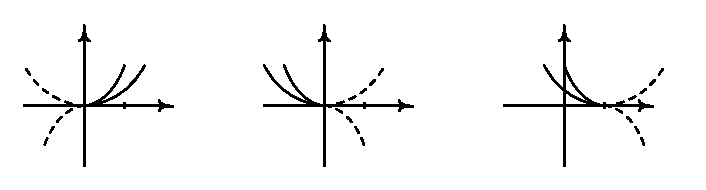
\includegraphics[scale=1.25]{krivky_patocka_fxfmxfmxpb}\\
   % translate x=591 y=207 scale 0.30
   \putbox{0.65in}{1.06in}{1.20}{$f(x)$}%
   \putbox{1.19in}{0.40in}{1.20}{$x$}%
   \putbox{0.86in}{0.40in}{1.20}{$b$}%
   \putbox{2.65in}{1.06in}{1.20}{$f(-x)$}%
   \putbox{3.19in}{0.40in}{1.20}{$x$}%
   \putbox{2.86in}{0.40in}{1.20}{$b$}%
   \putbox{4.65in}{1.06in}{1.20}{$f(-x+b)$}%
   \putbox{5.19in}{0.40in}{1.20}{$x$}%
   \putbox{4.86in}{0.40in}{1.20}{$b$}%
   } % close 'parbox'
   } % close 'scalebox'
   \vspace{-\baselineskip} % this is not necessary, but looks better
